%
%  intro.tex
%
%  Created by Drew Conway on 2011-01-26
% 
%
\documentclass[xcolor=dvipsnames, 9pt]{beamer}

\usepackage{ulem}

\usepackage{amssymb}
\usepackage{amsfonts}
\usepackage{amsmath}
\usepackage{hyperref}
\usepackage{natbib}
\usepackage{color}
\usepackage{pdfsync}
\usepackage{chancery}
\usepackage{movie15}
\usepackage{pgfpages}
\usepackage{fancyvrb}
\usepackage{colortbl}
\usepackage{multirow}

\usepackage{graphicx}
\graphicspath{{../../images/figures/}{../../images/logos/}{../../images/graphs/}/}

\usepackage{beamerthemesplit}
\usetheme{Copenhagen}
\definecolor{title}{RGB}{128,148,182}
\usecolortheme[named=title]{structure} 
\setbeamertemplate{headline}{}
\setbeamertemplate{navigation symbols}{}
\setbeamertemplate{itemize items}[triangle]
\setbeamertemplate{enumerate items}[default]
\setbeamertemplate{footline}[page number]{}
%\setbeameroption{show notes on second screen}


\usepackage{listings}
%\usepackage{listings,arev}
\definecolor{keywords}{RGB}{128,148,182}
\definecolor{comments}{RGB}{60,179,113}
\lstset{numbers=left,
        showstringspaces=false,
        numberstyle=\tiny,
        %frame=leftline,
        numbersep=4.5pt,
  keywordstyle=\color{keywords}\bfseries,
  commentstyle=\color{YellowOrange}\emph
}

\newenvironment{code}{\begin{semiverbatim} \begin{footnotesize}}
{\end{footnotesize}\end{semiverbatim}}


\newcommand{\R}{\mathbb{R}}
\renewcommand{\d}{\mathsf{d}}
\newcommand{\dd}{\partial}
\newcommand{\E}{\mathsf{E}}
\newcommand{\bb}{\mathbf}

\title{Welcome to Data Bootcamp}
\author{Joseph Adler, Drew Conway, Jake Hofman, Hilary Mason}
\date{February 1, 2011}

\begin{document} 
    
\begin{frame}[plain]
  \titlepage 

  \tiny
  \href{http://creativecommons.org/licenses/by-sa/3.0/us/}{
\includegraphics[width=1cm]{ccbysa}}

  Creative Commons Attribution-Share Alike 3.0
\end{frame}


\begin{frame}[fragile]
    \frametitle{Speakers}
\begin{verbatim}
          @jadler, @hmason, @drewconway, @jakehofman
\end{verbatim}
    \vskip5pt
    \begin{center}
        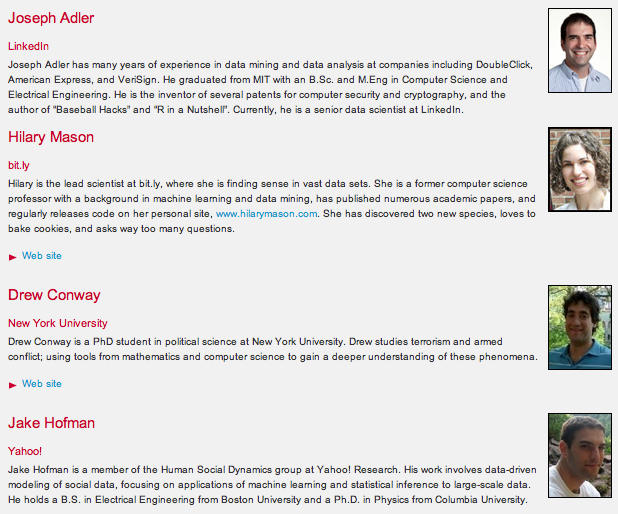
\includegraphics[width=0.775\textwidth]{speakers.png} \\
    \end{center}
\end{frame}


\section{Motivation for Bootcamp} % (fold)
\label{sec:motivation_for_bootcamp}

\begin{frame}[fragile]
    \frametitle{Please \textit{do} try this at home}
    All of the materials from today's tutorial are available on Github:
    \vskip20pt
    \begin{block}{Clone the repository for data/code/slides}
        \begin{lstlisting}[language=bash]
git clone https://github.com/drewconway/strata_bootcamp
        \end{lstlisting}
    \end{block}
\end{frame}


\begin{frame}[fragile]
  \frametitle{Disclaimer} % Disclaimer/Warning/Apologies
  
    You may be bored if you already know how to ...

      \begin{itemize}
        \item Acquire data from APIs
        \item Clean/explore/visualize data
        \item Classify and cluster image and text data
        \item Work with large data sets
        \item Build simple mashups
        \item Work with Python, R, SciPy/NumPy, etc.
        \item Work with unix tools on the command line, e.g.
      \end{itemize}

  \begin{verbatim}
    $ sed -e 's/<[^>]*>//g' < page.html > page.txt
  \end{verbatim}


%%   \begin{itemize}
%%     \item Scripting: Python, Ruby, Perl, bash, ...
%%     \item Computing: R, SciPy/NumPy, MATLAB, ...
%%     \item Wrangling: sed, awk, grep, tr, wc, cut, sort, uniq, ....
%%   \end{itemize}

%%   \begin{verbatim}
%%     $ tr , '\t' < data.csv > data.tsv
%%   \end{verbatim}

%%   \begin{verbatim}
%%     $ bzcat data.tsv.bz2 | awk -F'\t' 'NF != 16 {print}'
%%   \end{verbatim}

%%   \begin{verbatim}
%%     $ sed -e 's/<[^>]*>//g' < page.html > page.txt
%%   \end{verbatim}


\end{frame}





\begin{frame}
  \frametitle{Data-dependent products}

    \begin{center}
      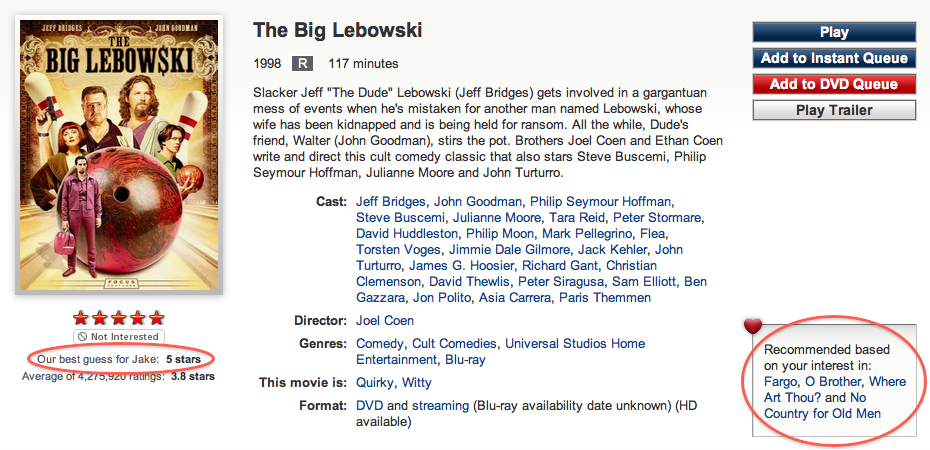
\includegraphics[width=\textwidth]{big_lebowski.png}
    \end{center}

    %\begin{itemize}
    %  \item \$1M for a 10\% improvement in predicted rating
    %\end{itemize}

\end{frame}


\begin{frame}
  \frametitle{Data-dependent products}

  \begin{itemize}
    \item Effective/practical systems that learn from experience impact our daily lives, e.g.:
      \begin{itemize}
        \item Recommendation systems
        \item Spam detection
        \item Optical character recognition
        \item Face recognition
        \item Fraud detection
        \item Machine translation
        \item $\ldots$
      \end{itemize}
  \end{itemize}

\end{frame}

\begin{frame}[fragile]
    \frametitle{Black\footnote{s/black/blue/g}-boxified?}
    \begin{center}
        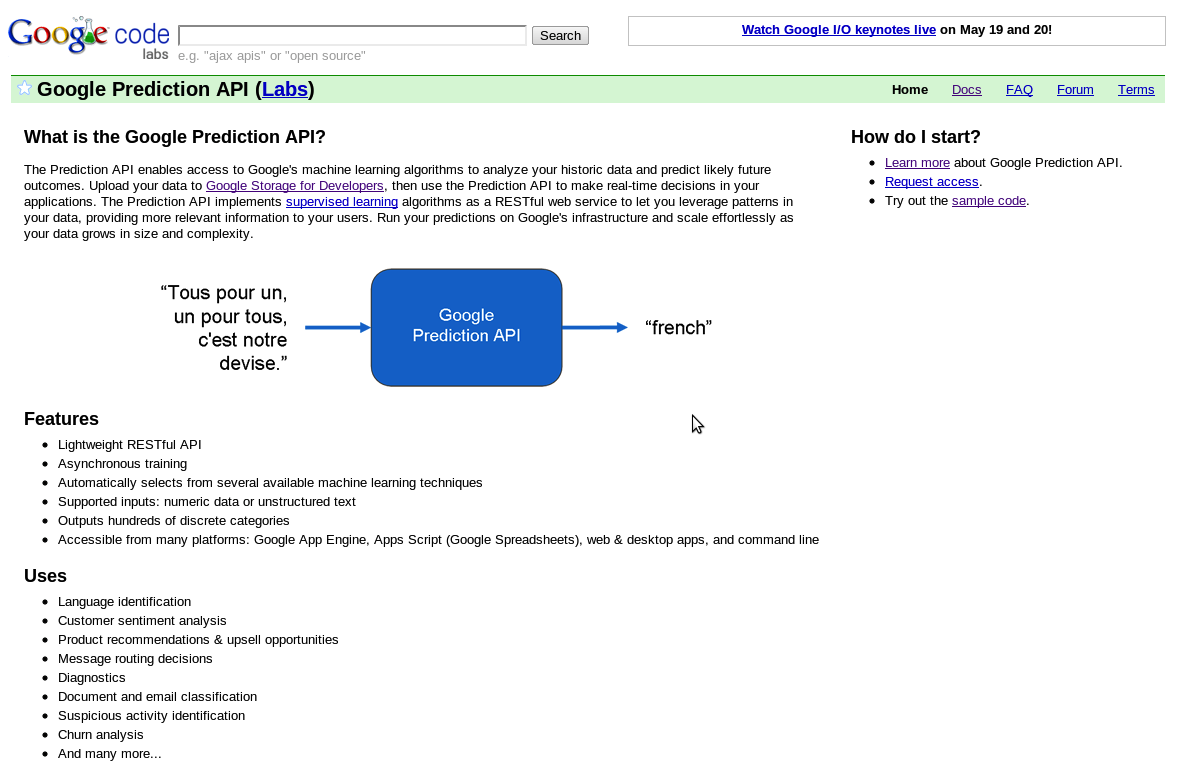
\includegraphics[width=0.9\textwidth]{google_pred_api.png}
    \end{center}
    % http://decisionstats.files.wordpress.com/2010/05/screenshot-15.png
\end{frame}


\begin{frame}
  \frametitle{Got data?}

  \begin{itemize}
    \item Web service APIs expose lots of data
  \end{itemize}

    \begin{center}
      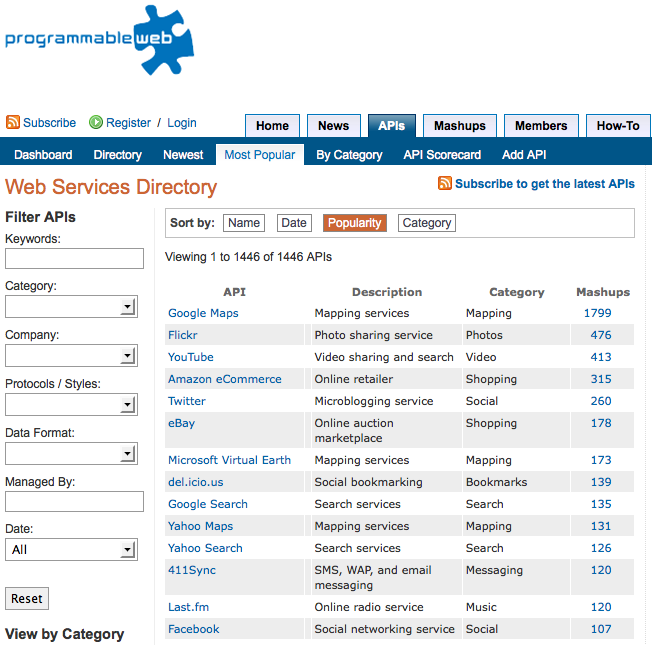
\includegraphics[width=0.625\textwidth]{programmableweb.png}
    \end{center}

\end{frame}

\begin{frame}
  \frametitle{Got data?}

  \begin{itemize}
    \item Many free, public data sets available online
  \end{itemize}

    \begin{center}
      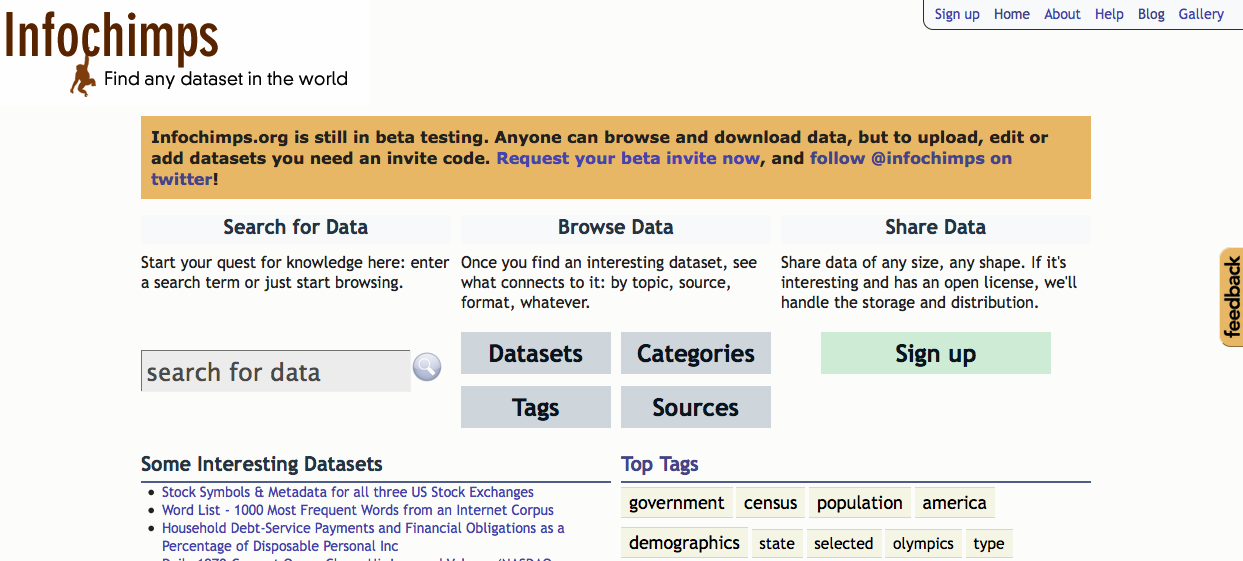
\includegraphics[width=0.9\textwidth]{infochimps.png}
    \end{center}

\end{frame}

\begin{frame}
  \frametitle{Roadmap?}

  \begin{columns}
    \column{0.4\textwidth}


    \column{0.3\textwidth}

    \begin{center}
      \Huge
      \begin{enumerate}
        \item[Step 1:] Have data
        \item[Step 2:] \alert{???}
        \item[Step 3:] Profit
      \end{enumerate}
    \end{center}

    \column{0.3\textwidth}

  \end{columns}

\end{frame}


\begin{frame}
  \frametitle{Learning by example}

    \begin{center}
      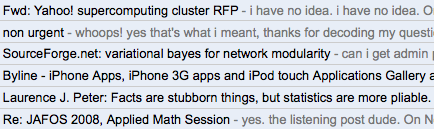
\includegraphics[width=0.75\textwidth]{email_ham.png}
      
\includegraphics[width=0.75\textwidth]{email_spam.png}
    \end{center}

    % s/rules/experience/
    \begin{itemize}
      \pause
      \item How did you solve this problem?
      \item \alert<2>{Can you make this process explicit (e.g. write code to do so)?}
    \end{itemize}

\end{frame}

\begin{frame}
  \frametitle{Learning by example}%s/rules/experience/}

    \begin{center}
      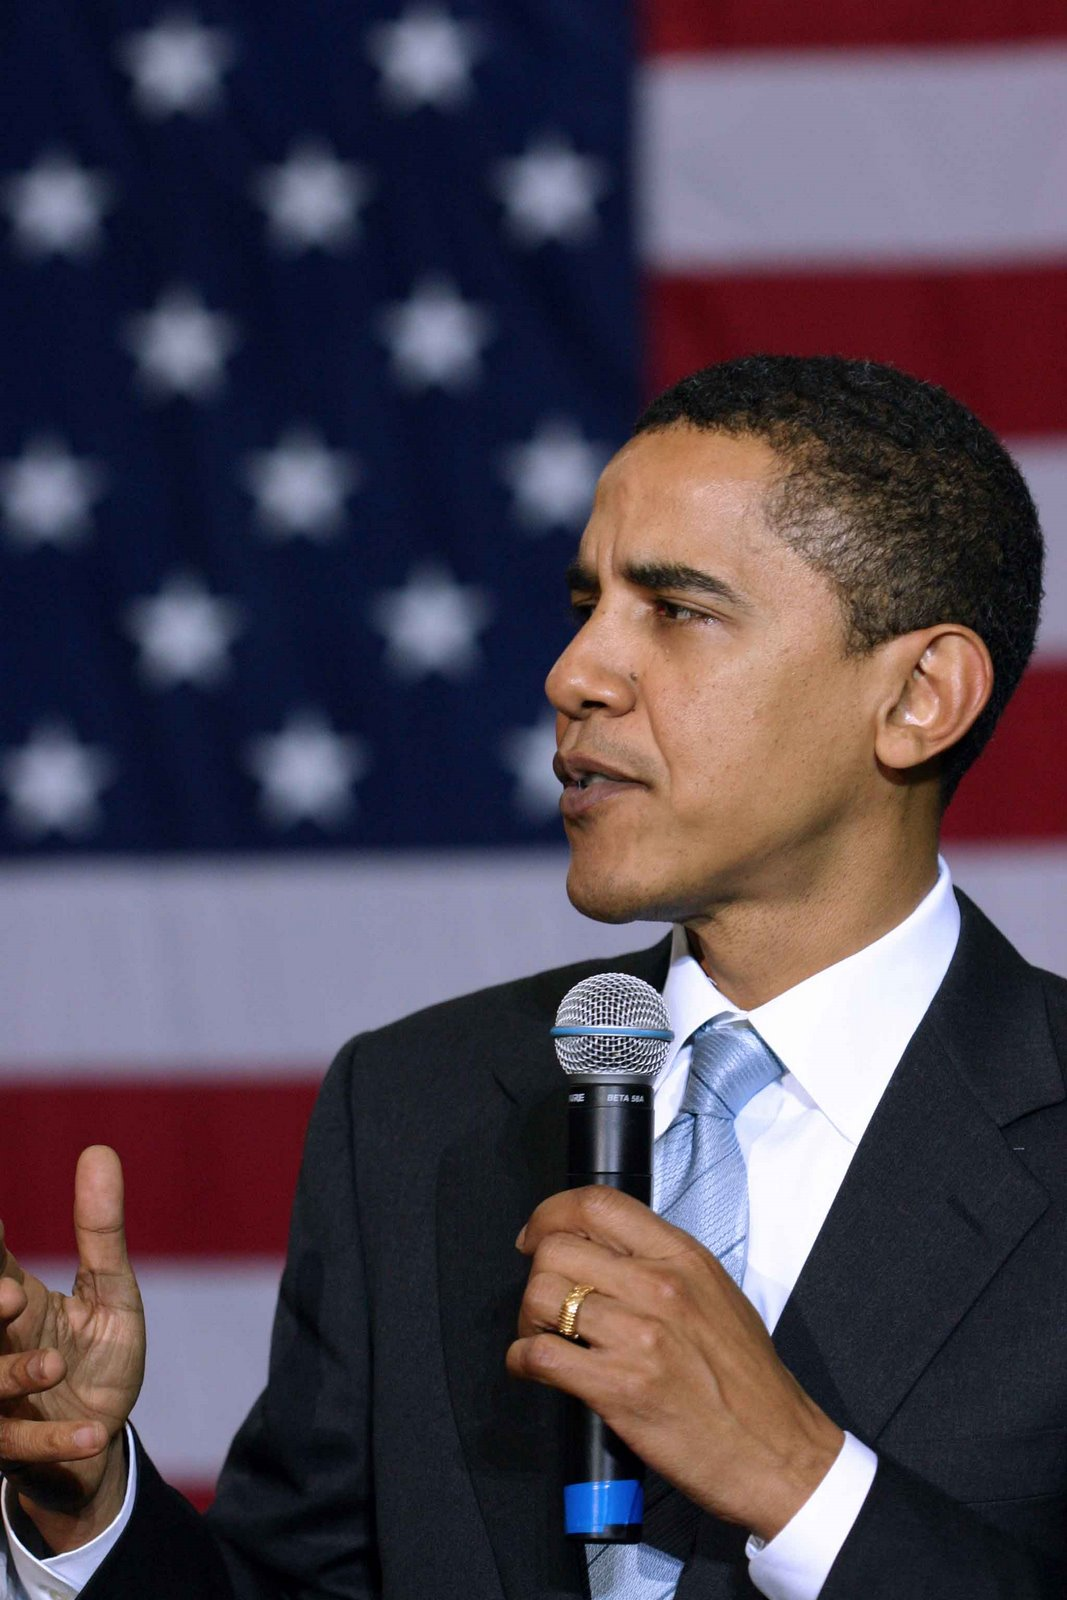
\includegraphics[width=0.25\textwidth]{obama1.png}
      
\includegraphics[width=0.25\textwidth]{obama2.png}
      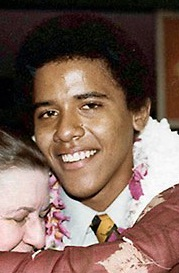
\includegraphics[width=0.25\textwidth]{obama4.png}
    \end{center}

    \begin{itemize}
      \item We learn quickly from few, relatively unstructured examples
       ... but we don't understand {\it how} we accomplish this
    \end{itemize}

\end{frame}




\begin{frame}
  \frametitle{Everything old is new again\footnote{\url{http://cbcl.mit.edu/publications/theses/thesis-rifkin.pdf}}}

  \begin{itemize}
    \item Many fields ...
      \begin{itemize}
        \item Statistics
        \item Pattern recognition
        \item Data mining
        \item Machine learning
      \end{itemize}
    \item ... similar goals
      \begin{itemize}
        \item Extract and recognize patterns in data
        \item Interpret or explain observations
        \item Test validity of hypotheses
        \item Efficiently search the space of hypotheses
        \item Design efficient algorithms enabling machines to learn from data
      \end{itemize}
  \end{itemize}

\end{frame}

\begin{frame}
  \frametitle{Statistics vs. machine learning\footnote{\url{http://anyall.org/blog/2008/12/statistics-vs-machine-learning-fight/}}}

    \begin{center}
      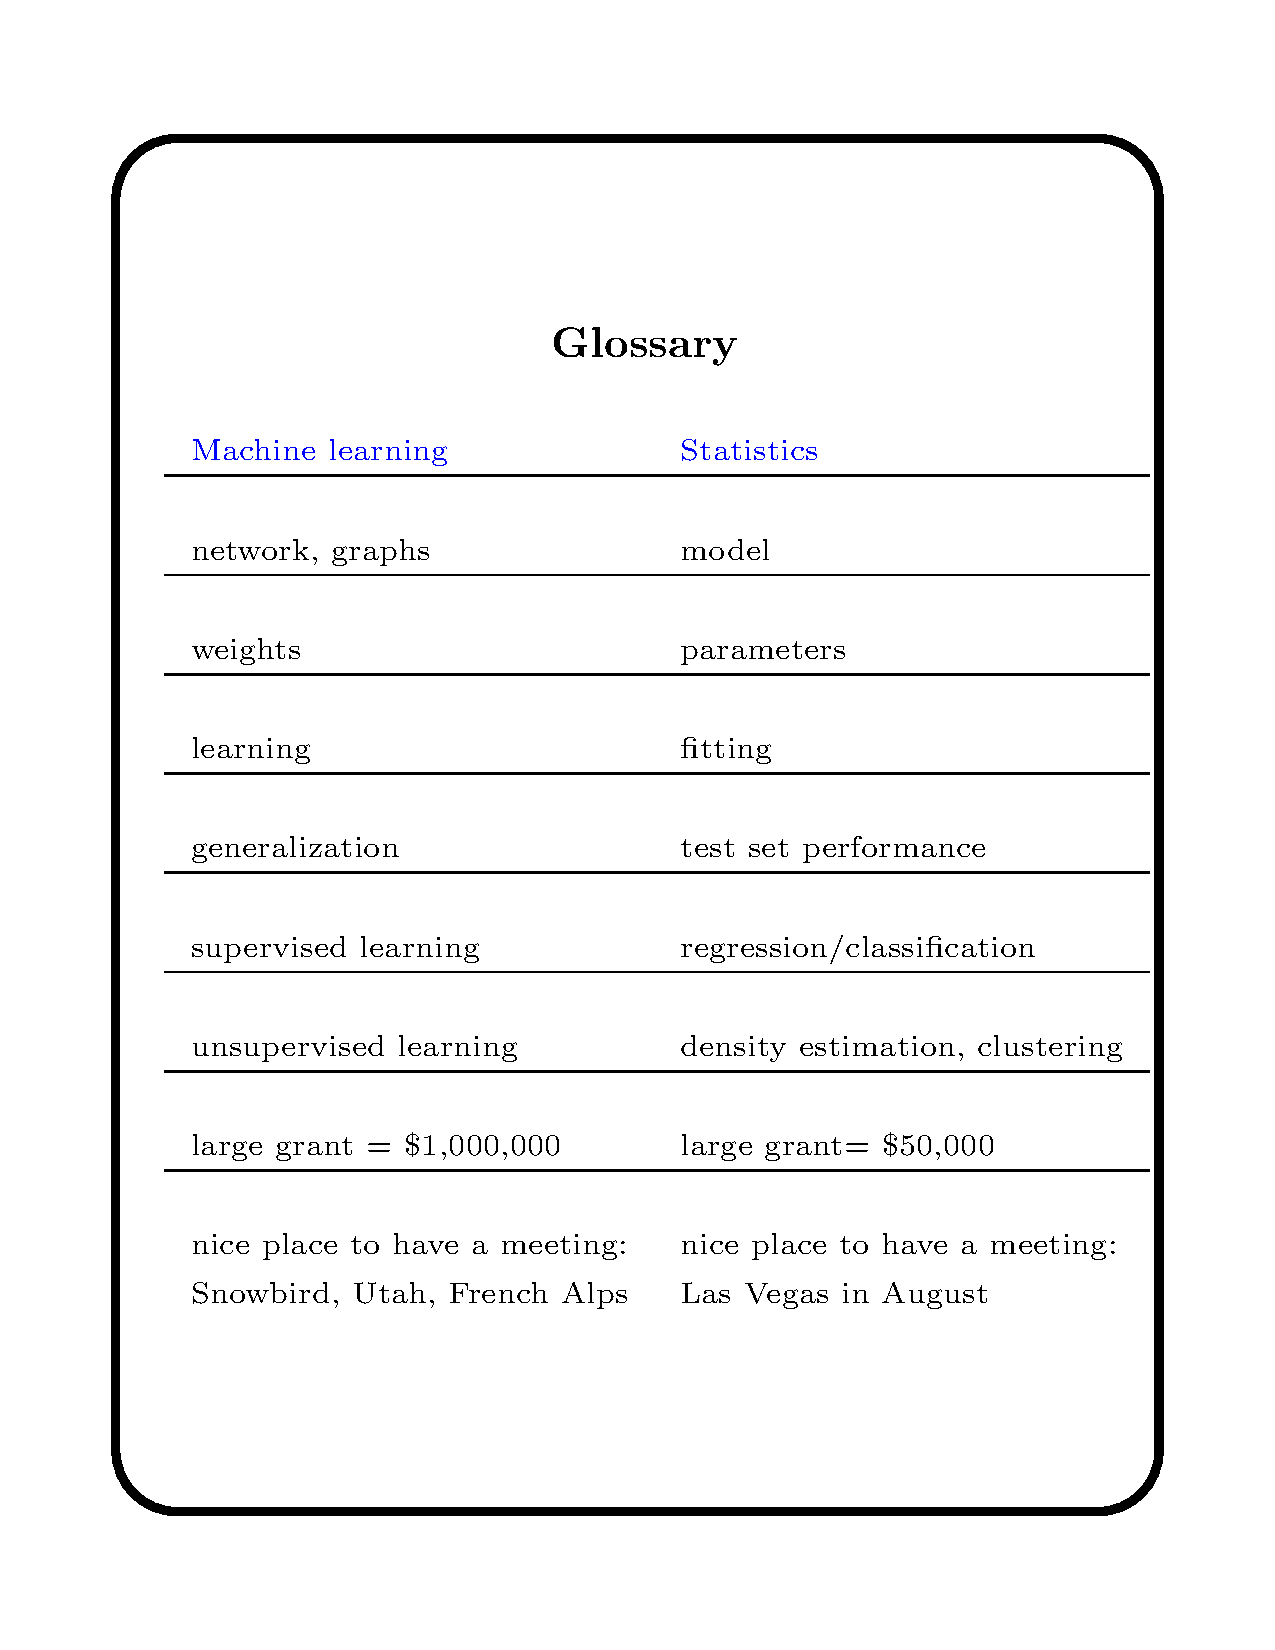
\includegraphics[height=0.825\textheight]{stat_vs_ml.pdf}
    \end{center}

\end{frame}



\begin{frame}
  \frametitle{Philosophy}

    \begin{itemize}
      \item We would like models that:
        \begin{itemize}
          \item Provide predictive and explanatory power
          \item Are complex enough to describe observed phenomena
          \item Are simple enough to generalize to future observations
        \end{itemize}

    \begin{center}
      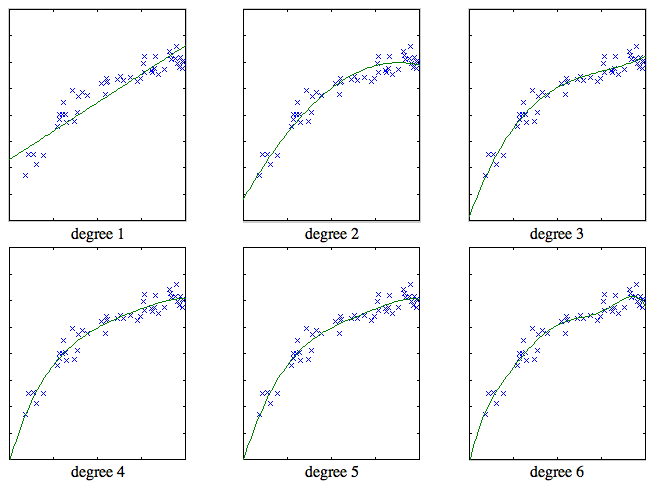
\includegraphics[width=0.5\textwidth]{regression.png}
    \end{center}

    \end{itemize}

\end{frame}



\begin{frame}
  \frametitle{Roadmap, take 2\footnote{\url{http://www.dataists.com/2010/09/a-taxonomy-of-data-science/}}}

  \begin{columns}
    \begin{column}{0.6\textwidth}
      
  \begin{enumerate}
    \item Get data
    \item Visualize/perform sanity checks
    \item Clean/filter observations
    \item Choose features to represent data
    \item Specify model
    \item Specify loss function 
    \item Develop algorithm to minimize loss 
    \item Choose performance measure
    \item ``Train'' to minimize loss
    \item ``Test'' to evaluate generalization
  \end{enumerate}

    \end{column}
    \begin{column}{0.3\textwidth}

    \begin{center}
      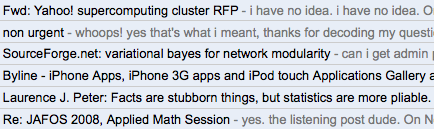
\includegraphics[width=0.9\textwidth]{email_ham.png}
      
\includegraphics[width=0.9\textwidth]{email_spam.png}
      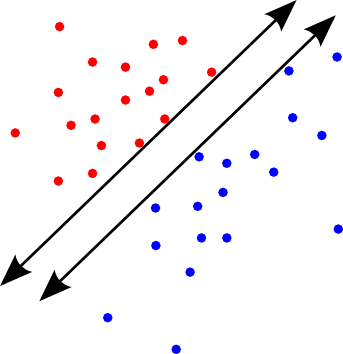
\includegraphics[width=0.5\textwidth]{svm.png}
      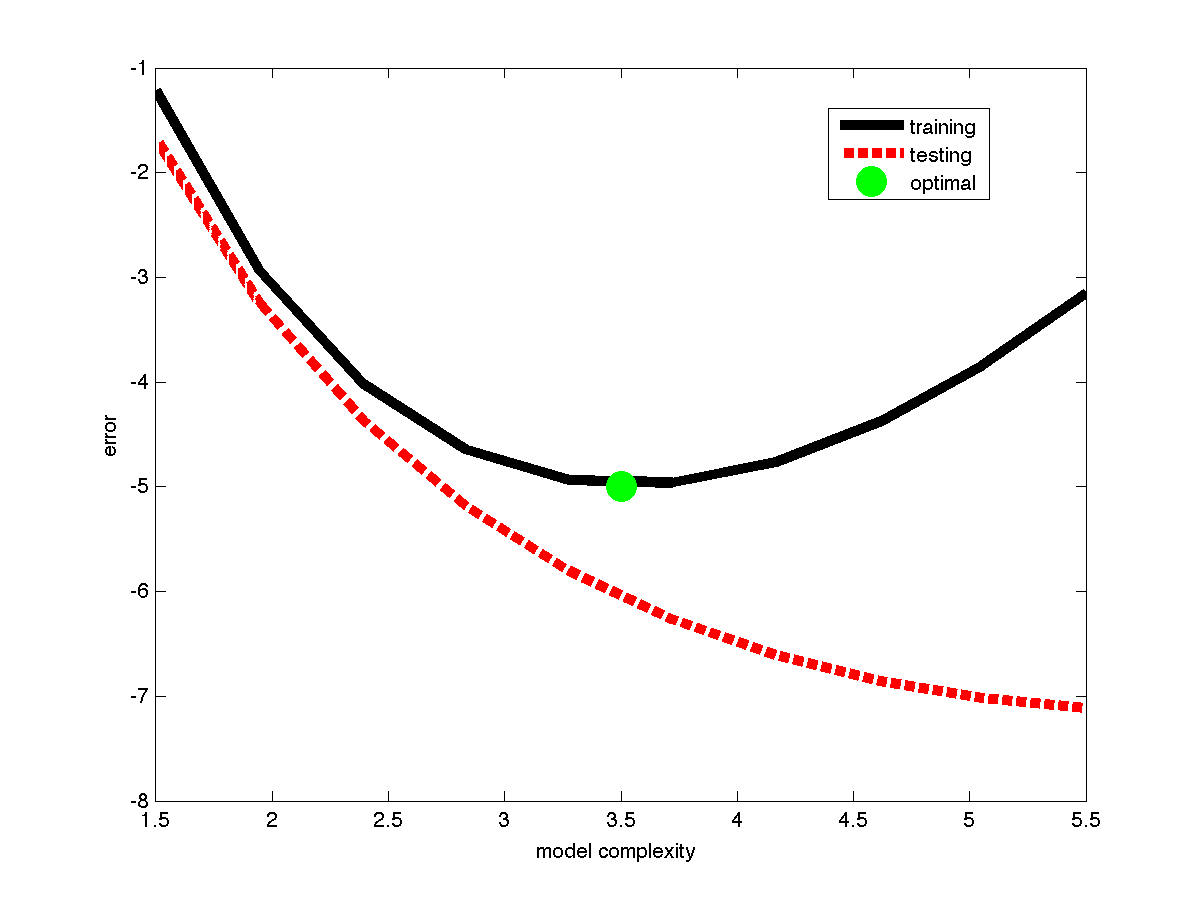
\includegraphics[width=0.9\textwidth]{complexity.png}
    \end{center}

    \end{column}
  \end{columns}
\end{frame}


\begin{frame}
  \frametitle{Roadmap, take 3}

    \begin{center}
      
\includegraphics[width=0.9\textwidth]{netflix_faq.png}
      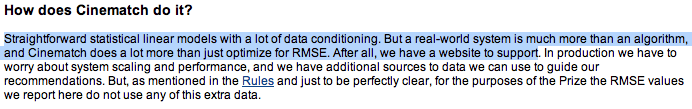
\includegraphics[width=0.9\textwidth]{netflix_cinematch.png}
    \end{center}

\end{frame}


\begin{frame}
  \frametitle{Shipping = Feature}

    \begin{center}
      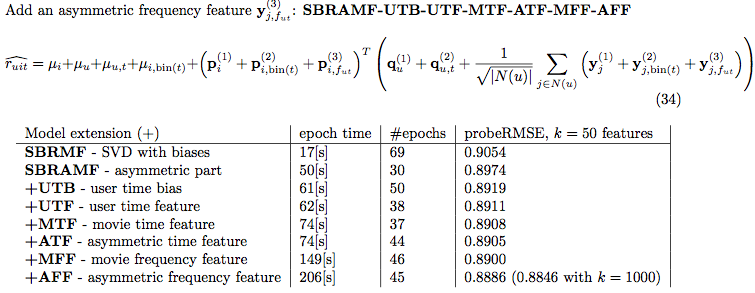
\includegraphics[width=0.8\textwidth]{netflix_solution.png}
    \end{center}

\end{frame}

\begin{frame}
  \frametitle{Themes}


 \begin{center}
  \structure{
    \only<1>{Data jeopardy}
    \only<2-4>{Data hacking}
    \only<5-6>{Data ``science''}
  }

  \vskip20pt

  \only<1> {
    Regardless of scale, it's difficult to find the right
    questions to ask of the data
    }
  \only<2>{
    Cleaning and normalizing data is a substantial amount of the
    work (and likely impacts results)
  }
  \only<3>{
    The ability to iterate quickly, asking and answering many
    questions, is crucial
  }
  \only<4>{
    Hacks happen: sed/awk/grep are useful, and scale
  }
  \only<5>{
    Simple methods (e.g., linear models) work surprisingly well, especially with lots of data
    % Simple methods often work surprisingly well, especially for large problems
  }
  \only<6>{
    It's easy to cover your tracks---things are often much more complicated than they appear
    %and make things appear easier than they were
  }

 \end{center}



\end{frame}


\begin{frame}
  \frametitle{References}

    \begin{center}
      
\includegraphics[width=0.3\textwidth]{seagaran.png}
      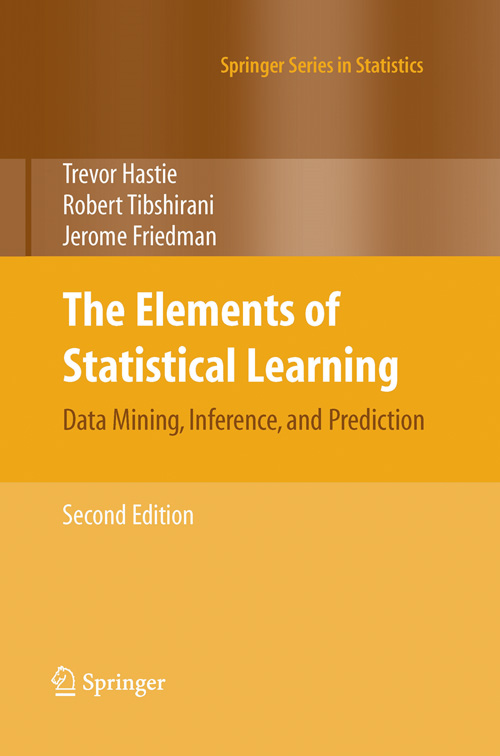
\includegraphics[width=0.3\textwidth]{hastie.jpg}
      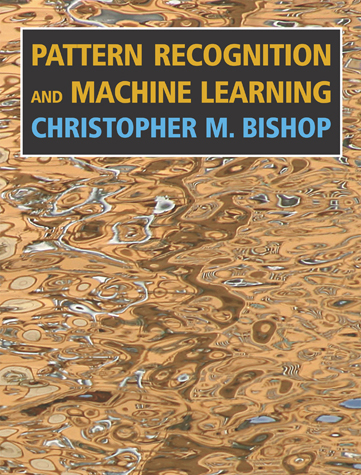
\includegraphics[width=0.3\textwidth]{bishop.jpg}
    \end{center}
\end{frame}


% section motivation_for_bootcamp (end)

\end{document}
